\SSbreak\\
\emph{Source: Italian Team Competition}\\
\emph{Proposer: \Phobo}\\ %\Pchan \Pbrain \Pss
\emph{Problem ID: 220}\\
\emph{Date: 2021-06-30}\\
\emph{Difficulty: Medium}\\
\SSbreak

\SSpsetQ{
    Diagonals of parallelogram $NJSM$ interescts at $E$, angle bisectors of $\angle MNE$ and $\angle EJS$ intersects at $L$. Given that $MESL$ is a parallelogram and $\overline{NM}=35$, compute $\overline{NJ}^2$.
    %Put Problem Here
}\bigskip

\begin{solution}\hfil\medskip
	
    Note $NS\parallel ML$ so $\angle NLM=\angle LNE = \angle MNL$ which makes $\triangle MNL$ isosceles, hence $\overline{MN} = \overline{ML}=\overline{ES}$. With a similar reasoning we get $\triangle JSL$ isoceles, with $\overline{JS}=\overline{SL}=\overline{EM}$, but $\overline{MN}=\overline{JS}$ so $\overline{EM}=\overline{ES}$, but recalling $E$ is the midpoint of both diagonals, $\overline{NS}=\overline{JM}$, making $NJSM$ a rectangle. Now $\overline{MJ}=2\cdot\overline{MN}$, which gives $\overline{NJ}=\sqrt{3}\cdot \overline{NM}$, so finally $\overline{NJ}^2=3\cdot \overline{NM}^2=\boxed{3675}$.
    \begin{figure}[h!]
        \centering
    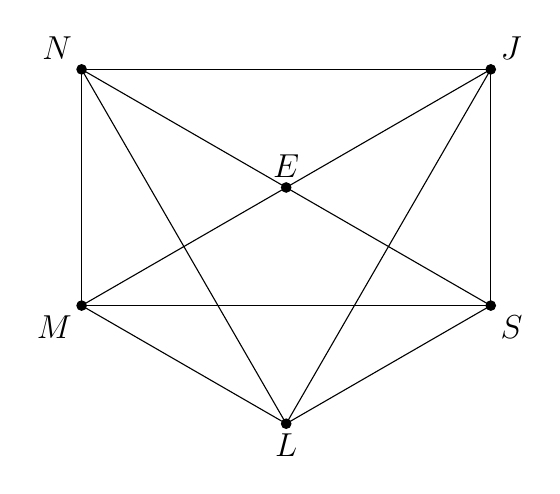
\begin{tikzpicture}[scale=3]
    \def\N{(0,1)};
    \def\J{(1.73205080757,1)};
    \def\S{(1.73205080757,0)};
    \def\M{(0,0)};
    \def\E{(0.86602540378,0.5)};
    \def\L{(0.86602540378,-0.5)};
    \draw \N -- \J -- \S -- \M -- \N;
    \draw \N -- \S -- \L -- \M -- \J -- \L -- \N;
    \filldraw \N circle (0.02) node[above left] {\large $N$};
    \filldraw \J circle (0.02) node[above right] {\large $J$};
    \filldraw \S circle (0.02) node[below right] {\large $S$};
    \filldraw \M circle (0.02) node[below left] {\large $M$};
    \filldraw \E circle (0.02) node[above] {\large $E$};
    \filldraw \L circle (0.02) node[below] {\large $L$};
    \end{tikzpicture}
    \end{figure}
    %Put sol here
\end{solution}\bigskip